%% VEGABrain -- manuscript for Neuroinformatics (Springer)
%% Springer Nature journal article template v3.1 (December 2024).
%% Reference style: sn-basic (author-year), which is what Neuroinformatics uses.
%% Build:  bash build.sh      (see IMPLEMENTATION.md)
%%
%% Add the "lineno" option below when producing the copy for reviewers:
%%   \documentclass[lineno,pdflatex,sn-basic]{sn-jnl}

\documentclass[pdflatex,sn-basic]{sn-jnl}

%%%% Standard Packages
\usepackage{graphicx}%
\usepackage{amsmath,amssymb,amsfonts}%
\usepackage{xcolor}%
\usepackage{textcomp}%
\usepackage{manyfoot}%
\usepackage{booktabs}%
\usepackage{tikz}%
\usetikzlibrary{arrows.meta,positioning}%
\usepackage{url}%
%%%%

\graphicspath{{figures/}}
\raggedbottom

\begin{document}

\title[VEGABrain]{VEGABrain: a Visualizer of Enriched Gene Analysis for the
developing human brain}

%% TODO(authors): confirm author order, add ORCIDs via \orcid{...} inside \author,
%% and replace the affiliation placeholders with the full postal address of the
%% MCB Lab / department at UFRN.

\author[1]{\fnm{Isaac} \sur{Medeiros}}\email{isaac.medeiros.112@ufrn.edu.br}

\author[1]{\fnm{Jo\~{a}o V.} \sur{F. Cavalcante}}\email{joao.cavalcante.073@ufrn.edu.br}

\author*[1]{\fnm{Diego} \sur{Marques-Coelho}}\email{diego.marques.135@ufrn.edu.br}

\affil*[1]{\orgdiv{Bioinformatics Multidisciplinary Environment}, \orgname{Federal University of Rio Grande do Norte}, \orgaddress{\street{Rua do Horto}, \city{Natal}, \postcode{59076-550}, \state{Rio Grande do Norte}, \country{Brazil}}}

%%==================================================================%%
%% Abstract
%%==================================================================%%

\abstract{
  RNA sequencing datasets are widely reused resources in developmental neuroscience, yet inspecting them spatially remains unclear and difficult. Here, we present VEGABrain, an openly accessible web tool that renders bulk RNA-seq onto brain cortical and subcortical atlas surfaces across five human developmental windows spanning the first trimester to adulthood. Beyond single-gene maps, VEGABrain contributes a composite per-region enrichment layer using single-sample gene set enrichment analysis (ssGSEA) scores precomputed for ${\sim}$19,000 gene sets drawn from Gene Ontology, Reactome, KEGG, BioCarta, the Human Phenotype Ontology and the MSigDB hallmark collection, and aggregated to a score for every gene set, developmental window and brain region. Furthermore, VEGABrain allows users to submit a custom gene list and obtain its ssGSEA map across development, computed on demand. VEGABrain is open source and requires no installation, offering easy-to-query expression throughout development and brain areas.
}

\keywords{Neuroinformatics, Brain development, BrainSpan, Gene set enrichment,
ssGSEA, Data visualization, Web application}

\maketitle

%%==================================================================%%
\section{Introduction}\label{sec:intro}
%%==================================================================%%

The transcriptome of the developing human brain is one of the most heavily
reused datasets in neuroscience. The BrainSpan atlas
\citep{BrainSpan2011,Kang2011,Miller2014} sampled bulk tissue from cortical and
subcortical structures across prenatal and postnatal donors, and subsequent
integrative work built on it to relate developmental expression to
neuropsychiatric risk \citep{Li2018} and to evolutionary divergence between
human and macaque \citep{Zhu2018}.

What has not kept pace is the ease of seeing it. A researcher who wants
to know where and when a gene, or a set of genes, is expressed in the developing
brain has essentially two options today, and both impose costs that are
unrelated to the biological question.

The first is the resource portal. Portals in this family---BrainSpan itself, and
the wider family of Allen Institute browsers \citep{Lau2008,Sunkin2013}---return
the data as tables, line plots or heat maps indexed by structure acronym. This, unfortunately, is 
not anatomical: the reader must hold the mapping from
\texttt{DFC}, \texttt{MFC} or \texttt{STC} to a location in the brain, 
and a heat map of 26 structure codes does not convey a spatial gradient
the way a rendered cortex does. It is also gene-at-a-time. There is no route
from a gene set, a pathway, or the output of a differential-expression analysis
to a spatial view. Newer hosted portals have narrowed part of this gap:
BrainScope links genes and samples through t-SNE maps to choropleths over
anatomical slices \citep{Huisman2017}, and SMDB browses spatial transcriptomic
data in two and three dimensions \citep{Cao2023}. Neither, however, scores a
gene set across a human developmental parcellation
(Section~\ref{sec:comparison}).

The second option is to do it yourself. Excellent programmatic brain-plotting
tools exist---\texttt{ggseg} and \texttt{ggseg3d} \citep{Mowinckel2020} and
\texttt{cerebroViz} \citep{Bahl2017} in R, \texttt{neuromaps} in Python
\citep{Markello2022}, and \texttt{abagen} for the adult Allen Human Brain Atlas
\citep{Hawrylycz2012,Markello2021}. But that route presupposes a user who
writes R or Python, who is willing to download and hold a $52{,}376 \times 524$
expression matrix locally, and who will construct and validate the mapping from
BrainSpan's tissue nomenclature onto an atlas parcellation. Each of those steps
is a place where a project stalls or a mapping silently diverges between
laboratories \citep{Markello2021}.

Additionally, modern analyses rarely end
with one gene. They end with a list, be it a differentially expressed set, a module
from a co-expression network or a panel of risk genes for a disorder. The natural
question is then not ``where is gene $X$ expressed?'' but ``where and when is
this programme active?''. Answering it requires collapsing many genes
into a single per-sample summary. Single-sample gene set enrichment analysis
(ssGSEA) \citep{Barbie2009}, a per-sample variant of GSEA
\citep{Subramanian2005} implemented alongside GSVA \citep{Hanzelmann2013},
provides exactly such a composite score, and has been used as a quantitative
readout of pathway activity in expression data
\citep{Yi2020}. The incorporation of composite multigene activity scores (such as those generated by ssGSEA or GSVA) into anatomical models directly addresses the challenge of condensing high-dimensional expression profiles into interpretable summaries, ensuring noise reduction and dimensionality reduction compared to classical single-gene-based analyses \citep{Hanzelmann2013}. To our knowledge no tool has applied it as a
\emph{spatial} layer over the developing human brain.

VEGABrain (Visualizer of Enriched Gene Analysis) addresses these three gaps in
one interface, reachable at \url{https://mcblab.github.io/BrainMap/} with no
installation, account or download. It maps BrainSpan samples onto cortical and
subcortical atlas parcels across five developmental windows; it adds a composite
enrichment layer of ssGSEA scores precomputed for 18{,}650 gene sets from the
Gene Ontology \citep{Ashburner2000,GOConsortium2023}, Reactome
\citep{Gillespie2022}, KEGG \citep{Kanehisa2000}, BioCarta, the Human Phenotype
Ontology \citep{Kohler2021} and the MSigDB hallmark collection
\citep{Liberzon2011,Liberzon2015}; and it scores user-submitted gene lists on
demand, closing the loop from an enrichment result \citep{Chen2013,Kuleshov2016}
back to anatomy. A submitted list may also carry log2 fold-change values from an
external comparison---a different disease model, treatment or condition---which
are then mapped against the BrainSpan expression data, so that analyses can
follow directions the dataset was not originally built for, not just the
comparisons already included in it. Both the maps and the numbers behind them are exportable, so
that VEGABrain is a starting point for downstream analysis, 
consistent with the FAIR principles for reusable research data
\citep{Wilkinson2016}.

%%==================================================================%%
\section{Materials and Methods}\label{sec:methods}
%%==================================================================%%

\subsection{Expression data and preprocessing}\label{sec:data}

VEGABrain is built on the BrainSpan Developmental Transcriptome RNA-Seq release,
Gencode v10 RPKM values summarised to genes \citep{BrainSpan2011,Miller2014}.
The distributed matrix contains 52{,}376 gene rows and 524 sample columns. Rows
with duplicate HGNC symbols are dropped, keeping the first occurrence, and
values are transformed as $\log_2(\mathrm{RPKM} + 1)$. No further normalisation
or batch correction is applied; the released RPKM values are used as the
provider distributes them, so that scores computed here remain comparable with
analyses performed directly on the public matrix. Preprocessing and the scoring
described in Section~\ref{sec:ssgsea} are performed once, offline
(Figure~\ref{fig:arch}).

\subsection{Developmental windows}\label{sec:ages}

BrainSpan donors span 31 distinct ages from 8 post-conceptional weeks to 40
years. Individual ages are too sparsely sampled to render as separate maps, so
donors are binned into five developmental windows: first trimester ($n=5$
donors), second trimester ($n=10$), third trimester ($n=5$), infant ($n=8$) and
adult ($n=14$). The donor counts are also given in Table~\ref{tab:data}; the
donor count is displayed in every facet label in the
interface so that the reader is never shown a map without also being shown how
much evidence stands behind it.

\subsection{Mapping BrainSpan structures to an atlas}\label{sec:mapping}

BrainSpan labels tissue by dissected structure (for example \emph{dorsolateral
prefrontal cortex}), whereas \texttt{ggseg} draws atlas parcels (for example
\emph{rostral middle frontal}). Cortical regions map onto the Desikan--Killiany parcellation
\citep{Desikan2006} and subcortical structures onto the FreeSurfer
\texttt{aseg} segmentation \citep{Fischl2002}, both accessed through
\texttt{ggseg} \citep{Mowinckel2020}.

Each atlas parcel is assigned a single BrainSpan structure. BrainSpan samples
far fewer structures than the atlases draw, so the assignment is many-to-one:
22 BrainSpan structures cover 42 atlas regions, and parcels that fall within
one dissected structure share its value (for example, the rostral and caudal
middle frontal parcels both take the dorsolateral prefrontal cortex samples).
Atlas regions with no BrainSpan counterpart, such as the brain stem, pallidum
and choroid plexus, are left unassigned. The complete assignment is a single
table distributed with the source code, so it can be inspected and changed
rather than reimplemented per project.

The interface exposes two levels of granularity. At the \emph{micro} scale each
of the 42 mapped atlas regions carries its own value. At the \emph{macro} scale
regions are pooled into six anatomical groupings---frontal, parietal, temporal
and occipital lobes, subcortical structures and cerebellum---the mean is taken
within each grouping, and that mean is painted back onto every region belonging
to it. The macro scale exists because BrainSpan sampling density varies sharply
across structures: pooling trades spatial resolution for donor support, and
letting the user switch between the two makes that trade-off explicit rather
than hidden. Regions with no corresponding sample are drawn in grey rather than
imputed.

Every map is rendered as four stacked panels---right lateral cortex, right
medial cortex, subcortical sagittal and subcortical coronal---each faceted into
the five developmental windows, giving a single figure in which spatial and
temporal structure are read on orthogonal axes.

\subsection{Composite enrichment scores}\label{sec:ssgsea}

For a gene set $G$ and a sample $j$, ssGSEA \citep{Barbie2009} ranks all genes
by their expression within that sample and computes an enrichment score from
the normalised difference between the empirical cumulative distribution of the
genes in $G$ and that of the genes outside it:

\begin{equation}\label{eq:ssgsea}
\mathrm{ES}(G, j) \;=\;
\sum_{i=1}^{N}\Bigl( P^{G}_{\mathrm{w}}(G, j, i) - P^{NG}(G, j, i) \Bigr),
\end{equation}

where $i$ indexes genes in decreasing order of expression in sample $j$,
$P^{G}_{\mathrm{w}}$ is the weighted cumulative distribution over genes in the
set and $P^{NG}$ the cumulative distribution over the rest. Because the score is
computed from within-sample ranks, it is invariant to the monotone
transformation applied in Section~\ref{sec:data} and does not require a
reference group or a phenotype contrast---which is what makes it usable here,
where each sample is a single donor--structure pair rather than a member of a
case/control design. We use the \texttt{ssgseaParam} interface of the
\texttt{GSVA} package \citep{Hanzelmann2013} with default parameters.

Gene sets are retrieved through \texttt{msigdbr} \citep{Dolgalev2025msigdbr} for
\emph{Homo sapiens} and comprise the MSigDB hallmark collection
\citep{Liberzon2015}, the canonical pathway subcollections BioCarta, KEGG
\citep{Kanehisa2000} and Reactome \citep{Gillespie2022}, and the full C5
ontology collection, which supplies Gene Ontology biological process, molecular
function and cellular component terms \citep{Ashburner2000,GOConsortium2023}
together with Human Phenotype Ontology terms \citep{Kohler2021}. The resulting
18{,}650 sets are broken down by collection in Table~\ref{tab:data}.

Scores are computed once for every gene set against all 524 samples, then
aggregated: for each (gene set, developmental window, region) triple the mean
score over the contributing samples is stored, and analogously for macro-regions,
so that an ontology query needs no enrichment run at request time. When instead a user submits their own gene list, the symbols are validated
against the matrix (unmatched symbols are reported back rather than silently
dropped), ssGSEA is run for that single set across all samples, and the same
aggregation is applied before rendering.

\subsection{Implementation}\label{sec:impl}

VEGABrain is an R \citep{RCoreTeam2026} service built with \texttt{plumber}
\citep{Schloerke2024plumber} behind a browser interface (Figure~\ref{fig:arch}).
Maps are rendered with \texttt{ggplot2} and \texttt{ggseg}
\citep{Mowinckel2020}, and can be downloaded as vector (SVG) figures together
with the per-region values behind them as CSV. The same service is exposed as a
public HTTP API, documented in the source repository, so that maps and tables
can also be retrieved programmatically.

%%------------------------------------------------------------------%%
%% Figure 1 -- data flow (drawn inline; no external asset)
%%------------------------------------------------------------------%%
\begin{figure}[htbp]
\centering
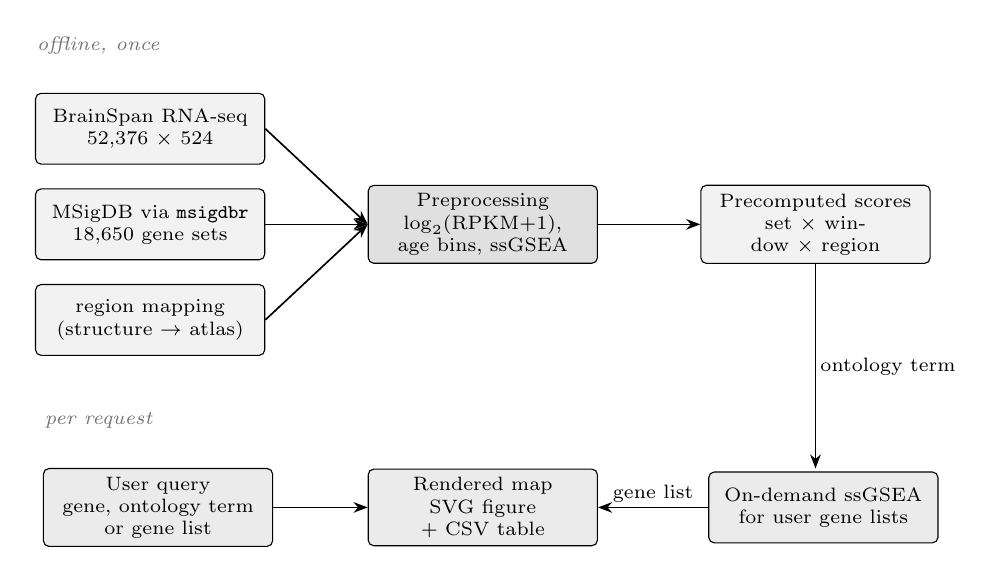
\begin{tikzpicture}[
  box/.style   = {draw, rounded corners=2pt, align=center, inner sep=3pt,
                  font=\scriptsize, minimum height=9mm, text width=27mm},
  data/.style  = {box, fill=black!5},
  proc/.style  = {box, fill=black!12},
  serve/.style = {box, fill=black!8},
  arr/.style   = {-{Stealth[length=1.8mm]}, semithick},
  lab/.style   = {font=\scriptsize, inner sep=1.5pt},
  band/.style  = {font=\scriptsize\itshape, text=black!55, anchor=west}
]
%% ---- offline band -------------------------------------------------
\node[data] (ms) {MSigDB via \texttt{msigdbr}\\18{,}650 gene sets};
\node[data, above=3mm of ms] (bs) {BrainSpan RNA-seq\\52{,}376 $\times$ 524};
\node[data, below=3mm of ms] (mp) {region mapping\\(structure $\rightarrow$ atlas)};

\node[proc, right=13mm of ms] (prep)
  {Preprocessing\\$\log_2(\mathrm{RPKM}{+}1)$,\\age bins, ssGSEA};
\node[data, right=13mm of prep] (rds)
  {Precomputed scores\\set $\times$ window $\times$ region};

\draw[arr] (bs.east) -- (prep.west);
\draw[arr] (ms.east) -- (prep.west);
\draw[arr] (mp.east) -- (prep.west);
\draw[arr] (prep) -- (rds);

%% ---- online band --------------------------------------------------
\node[serve, below=26mm of prep] (map)
  {Rendered map\\SVG figure $+$ CSV table};
\node[serve, left=12mm of map]  (user) {User query\\gene, ontology term\\or gene list};
\node[serve, right=14mm of map] (ondemand) {On-demand ssGSEA\\for user gene lists};

\draw[arr] (rds.south) -- node[lab, right] {ontology term} (rds.south|-map.north);
\draw[arr] (user) -- (map);
\draw[arr] (ondemand) -- node[lab, above] {gene list} (map);

\node[band] at ([yshift=6mm,xshift=-1mm]bs.north west) {offline, once};
\node[band] at ([yshift=6mm,xshift=-1mm]user.north west) {per request};
\end{tikzpicture}
\caption{VEGABrain data flow. The top row runs once, offline; the bottom row
runs per request. Ontology queries are served from the precomputed score table,
whereas a user-submitted gene list triggers a fresh ssGSEA run over all 524
samples.}
\label{fig:arch}
\end{figure}

%%==================================================================%%
\section{Results}\label{sec:results}
%%==================================================================%%

VEGABrain offers three query modes---a single gene, a precomputed ontology term,
or a user-submitted gene list---on a single working page.
All three produce the same four-panel, five-window
figure at either region granularity (Section~\ref{sec:mapping}), and a
reference map labelled by region name is available so that unfamiliar atlas
parcels can be identified. Every map can be exported together with the table of
values it was painted from, so a figure produced in VEGABrain and a statistic
computed from its export cannot disagree. We illustrate each mode with a case
whose developmental behaviour is independently established, so that the maps
can also be judged for biological face validity.

% TODO-measure: replace the qualitative statements below with the rendered maps
% and, where useful, the per-window means from the CSV exports.

\subsection{Single-gene maps}

Gene mode renders the mean $\log_2(\mathrm{RPKM}+1)$ of any gene in the matrix
per region and developmental window, on a fixed colour scale bounded at 6, so
that maps for different genes are directly comparable rather than each being
auto-scaled to its own range. Oligodendrocyte and myelination markers
(\emph{SOX10}, \emph{MBP}, \emph{PLP1}) should be low prenatally and rise
sharply in the infant and adult windows as myelination proceeds;
Figure~\ref{fig:gene} shows \emph{SOX10}. \textbf{[TODO: report the observed
per-window means]}.

\subsection{Gene-set maps}

Ontology mode returns the mean ssGSEA score of any of the 18{,}650 precomputed
gene sets per region and window (Figure~\ref{fig:ontology}). This is the
composite layer described in Section~\ref{sec:ssgsea}, and it is what
distinguishes VEGABrain from a gene-at-a-time browser: a single map summarises
the coordinated behaviour of tens to hundreds of genes. The member genes of the
selected set are listed alongside the map, so the composition of any score is
inspectable. Neurogenesis-associated terms such as
\texttt{GOBP\_FOREBRAIN\_GENERATION\_OF\_NEURONS} should peak in the prenatal
windows and decline postnatally; \textbf{[TODO]}. The composite score is
informative precisely here: the individual genes of a neurogenesis term are
noisy across 42 sparsely sampled regions, whereas the ssGSEA summary of the
term is not.

\subsection{User-submitted gene lists}

In gene-list mode, a pasted list of symbols is validated and scored on demand
(Figure~\ref{fig:genelist}). Symbols absent from the matrix are listed back to
the user explicitly, so a map is never quietly computed on a subset of what was
submitted. This is the path from an external result to anatomy: the output of a
differential expression analysis, a co-expression module, or a disorder risk
panel can be mapped across development directly, without the user preparing
data or writing code. GABAergic interneuron markers (\emph{GAD1}, \emph{GAD2},
\emph{SLC32A1}) should be present from the second trimester onward with
subcortical and then cortical distribution; \textbf{[TODO]}.In addition to entering genes, 
for each entry, the researcher can add a logFC value of their choice. The process can simulate 
how that variation in expression might impact the developmental process.

A further case tests the on-demand path against a model whose developmental
timing is experimentally fixed rather than merely presumed.
\citet{Fischer2021} exposed human pluripotent stem cells to chronic
intermittent ethanol throughout a 50-day differentiation to cortical neurons,
which corresponds to the first trimester, and report an upregulated
dorsal/glutamatergic specification programme. Submitting those 13 symbols
(Figure~\ref{fig:genelist}) through gene-list mode returns a map whose
region-averaged score declines monotonically across the five windows---0.81,
0.74, 0.58, 0.47, 0.44---so the signature is maximal in exactly the window the
\emph{in vitro} model represents, and the ordering is recovered from BrainSpan
alone, with no information from the original experiment. Because the exposure
window is part of the experimental design, this is a stronger test than a
disease with a merely prenatal attribution.

%%------------------------------------------------------------------%%
%% Figures 2-5 (placeholders in this draft -- see IMPLEMENTATION.md)
%%------------------------------------------------------------------%%

\begin{figure}[htbp]
\centering
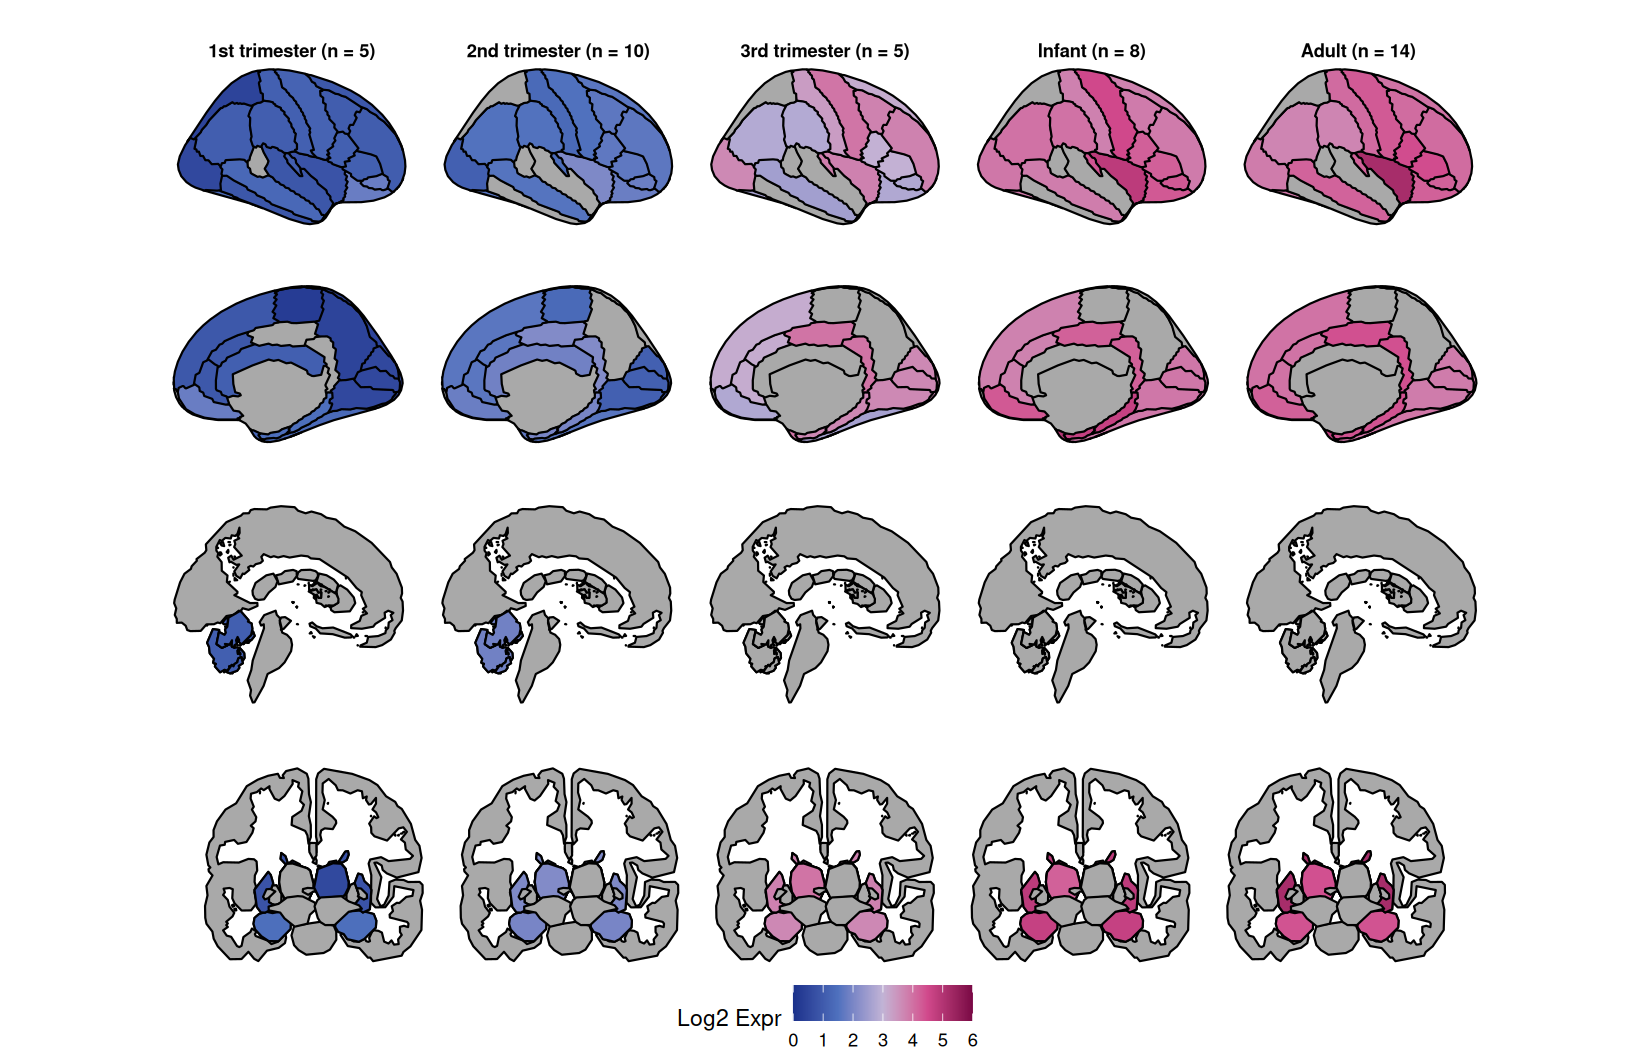
\includegraphics[width=\textwidth]{fig3_gene_sox10.png}
\caption{Single-gene mode. Mean $\log_2(\mathrm{RPKM}+1)$ for \emph{SOX10}
across the five developmental windows (columns) in four views (rows): right
lateral cortex and right medial cortex on the Desikan--Killiany parcellation,
and subcortical structures in sagittal and coronal section on the \texttt{aseg}
segmentation. Grey indicates regions with no BrainSpan sample in that window.}
\label{fig:gene}
\end{figure}

\begin{figure}[htbp]
\centering
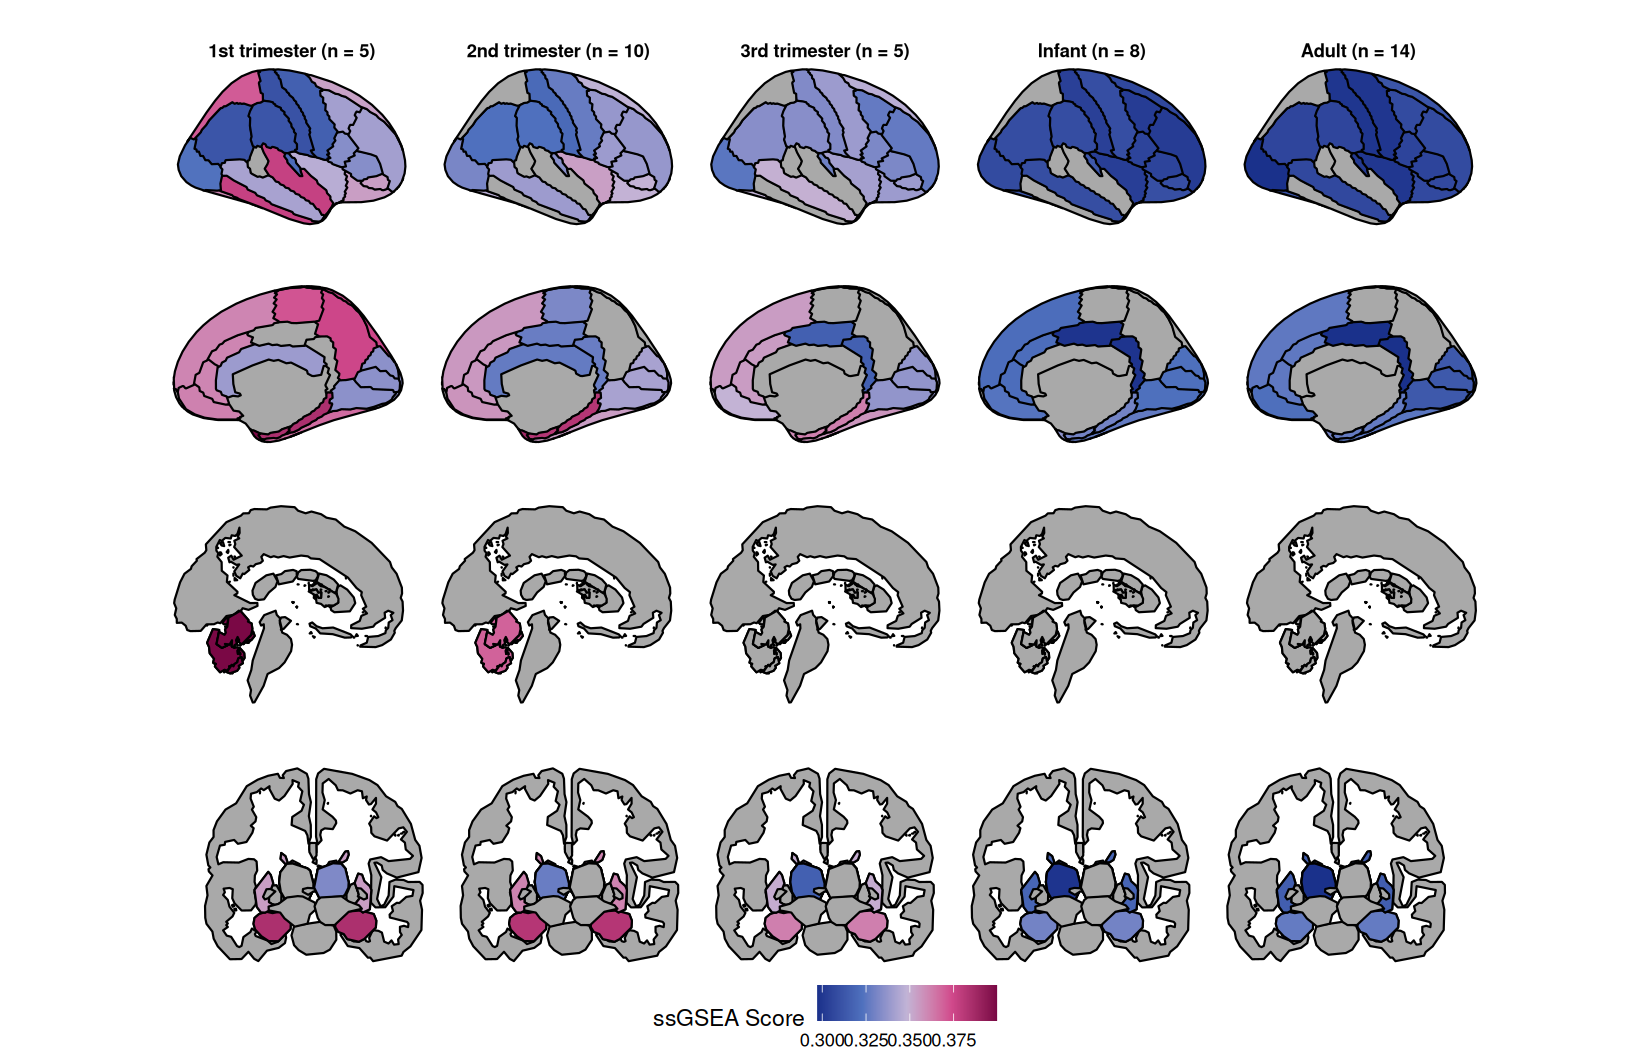
\includegraphics[width=\textwidth]{fig4_ontology.png}
\caption{Ontology mode: composite ssGSEA score for
\texttt{GOBP\_FOREBRAIN\_GENERATION\_OF\_NEURONS} across development. The score
summarises every gene in the term into one value per region and window; the same
term can be viewed at micro granularity (42 atlas regions) or macro granularity
(six anatomical groupings).}
\label{fig:ontology}
\end{figure}

\begin{figure}[htbp]
\centering
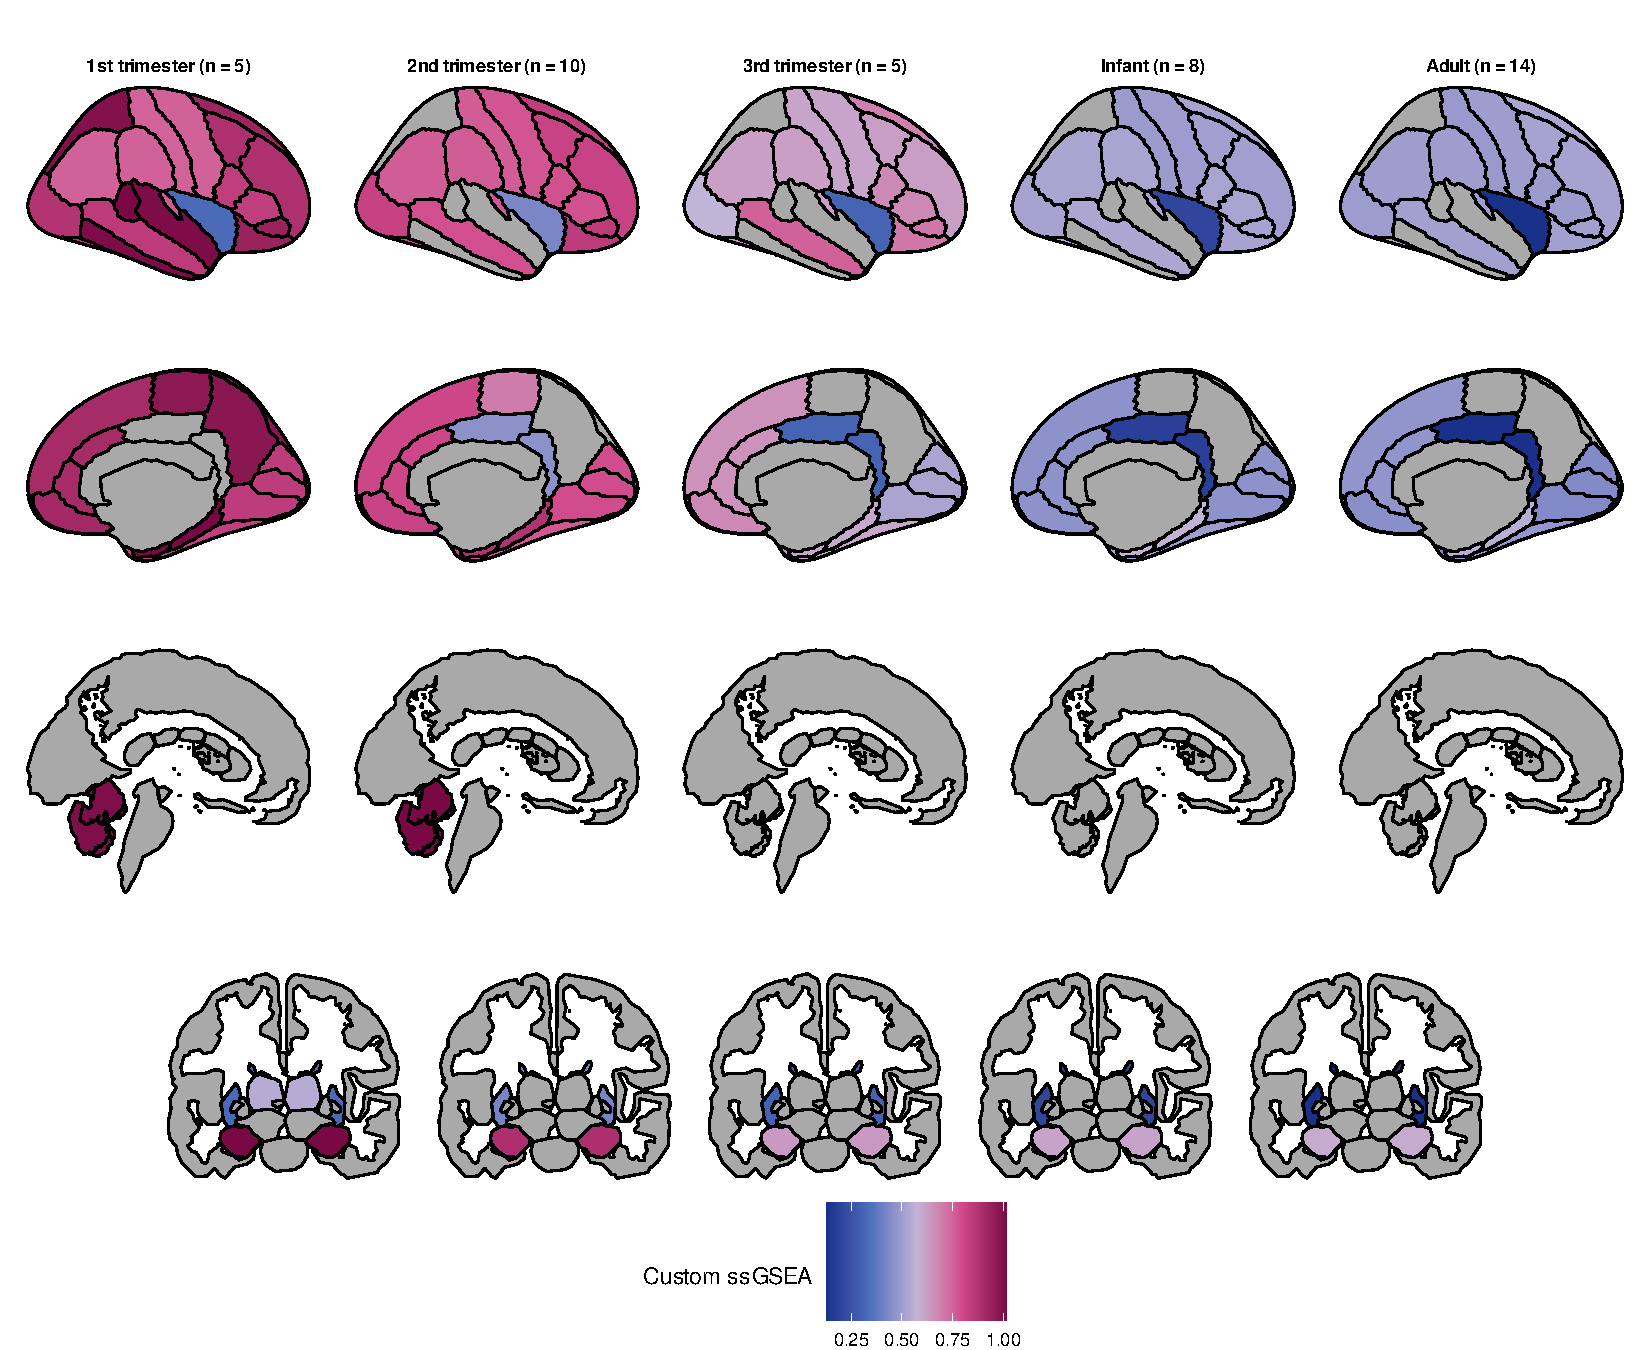
\includegraphics[width=\textwidth]{fig5_genelist.pdf}
\caption{User-submitted gene-list mode. ssGSEA computed on demand for the
dorsal/glutamatergic specification programme that \citet{Fischer2021} report as
upregulated by chronic intermittent ethanol exposure in human pluripotent stem
cells differentiated to first-trimester-equivalent cortical neurons
(\emph{EMX2}, \emph{LHX1/2/5/9}, \emph{OTX2}, \emph{FEZF2},
\emph{NEUROD1/2/6}, \emph{NEUROG2}, \emph{TBR1}, \emph{EOMES}). The submitted
list is a published differential-expression result, not a curated marker panel,
and it is mapped without local installation or coding. The score is highest in
the cortical parcels of the first two prenatal windows---the period the
\emph{in vitro} model corresponds to---and falls monotonically thereafter,
while the striatum stays low throughout, recovering the dorsal--ventral
contrast the signature encodes.}
\label{fig:genelist}
\end{figure}

%%------------------------------------------------------------------%%
%% Table 1 -- data summary
%%------------------------------------------------------------------%%
\begin{table}[htbp]
\centering
\caption{Data underlying VEGABrain.}\label{tab:data}
\begin{tabular}{@{}ll@{}}
\toprule
Property & Value \\
\midrule
Expression source        & BrainSpan RNA-Seq, Gencode v10 RPKM, gene-summarised \\
Matrix dimensions        & 52{,}376 genes $\times$ 524 samples \\
Transformation           & $\log_2(\mathrm{RPKM}+1)$; duplicate symbols dropped \\
Developmental windows    & 5 (see below) \\
\quad 1st trimester      & 5 donors \\
\quad 2nd trimester      & 10 donors \\
\quad 3rd trimester      & 5 donors \\
\quad Infant             & 8 donors \\
\quad Adult              & 14 donors \\
Atlas regions (micro)    & 42 (Desikan--Killiany cortical + \texttt{aseg} subcortical) \\
Anatomical groups (macro)& 6 (frontal, parietal, temporal, occipital, subcortical, cerebellum) \\
Views per map            & 4 (DK lateral, DK medial, \texttt{aseg} sagittal, \texttt{aseg} coronal) \\
Gene sets scored         & 18{,}650 total \\
\quad GO biological process & 7{,}538 \\
\quad Human Phenotype Ontology & 5{,}793 \\
\quad GO molecular function & 1{,}872 \\
\quad Reactome           & 1{,}839 \\
\quad GO cellular component & 1{,}080 \\
\quad BioCarta           & 292 \\
\quad KEGG (legacy)      & 186 \\
\quad MSigDB hallmark    & 50 \\
\botrule
\end{tabular}
\end{table}

%%==================================================================%%
\section{Discussion}\label{sec:discussion}
%%==================================================================%%

VEGABrain lowers the cost of asking a spatial question of the developing human
transcriptome from a small project to a few seconds in a browser. The composite enrichment layer extends the same reasoning to the
unit that modern analyses actually produce---a gene set---and the on-demand mode
means a user's own list is a first-class input rather than something the tool's
authors had to anticipate.

\subsection{Relation to existing tools}\label{sec:comparison}

Table~\ref{tab:compare} positions VEGABrain against the tools a researcher would
otherwise reach for. The comparison is deliberately along axes of \emph{what the
user must supply}, not of raw capability: each of these tools is stronger than
VEGABrain in its own domain, and the point is that none of them closes the
particular path VEGABrain is built for---from a gene set to a scored,
parcellated map of the developing brain, in a browser.

\begin{table}[htbp]
\centering
\caption{VEGABrain relative to comparable tools. \checkmark{} = supported,
--- = not supported or out of scope.}\label{tab:compare}
\footnotesize
\setlength{\tabcolsep}{4pt}
\begin{tabular}{@{}p{44mm}ccccc@{}}
\toprule
& Developmental & Anatomical & Gene-set & Custom list & No install \\
& axis & rendering & scoring & input & required \\
\midrule
VEGABrain (this work)             & \checkmark & \checkmark & \checkmark & \checkmark & \checkmark \\
BrainSpan portal \citep{BrainSpan2011} & \checkmark & ---   & ---        & ---        & \checkmark \\
Allen browsers \citep{Lau2008,Sunkin2013} & ---   & \checkmark & ---     & ---        & \checkmark \\
BrainScope \citep{Huisman2017}         & \checkmark & \checkmark & ---   & \checkmark & \checkmark \\
SMDB \citep{Cao2023}                   & ---        & \checkmark & ---   & ---        & \checkmark \\
\texttt{ggseg} \citep{Mowinckel2020}   & ---        & \checkmark & ---   & \checkmark & --- \\
\texttt{neuromaps} \citep{Markello2022}& ---        & \checkmark & ---   & \checkmark & --- \\
\texttt{abagen} \citep{Markello2021}   & ---        & \checkmark & ---   & \checkmark & --- \\
\texttt{cerebroViz} \citep{Bahl2017}   & \checkmark & \checkmark & ---   & \checkmark & --- \\
Programmatic plotting guides \citep{Chopra2023} & --- & \checkmark & --- & \checkmark & --- \\
Enrichr \citep{Chen2013,Kuleshov2016}  & ---        & ---        & \checkmark & \checkmark & \checkmark \\
\texttt{VoxHunt} \citep{Fleck2021}     & \checkmark & \checkmark & ---   & \checkmark & --- \\
\botrule
\end{tabular}
\footnotetext{``Developmental axis'' means the tool natively presents variation
across prenatal-to-postnatal time. ``Anatomical rendering'' means values are
drawn onto a picture of the brain, in whatever form the tool adopts---a
parcellated surface, a slice choropleth or a three-dimensional point cloud.
``Gene-set scoring'' means it produces a composite per-sample score for a set of
genes rather than plotting genes individually; a tool that displays the mean
expression of a set, or that hands the set to an external enrichment server,
does not qualify. ``Custom list input'' means the user may supply their own
genes or their own per-region values.}
\end{table}

As noted in the Introduction, the portals are gene-at-a-time and the
programmatic tools take a value per region as \emph{input}, leaving the user to
obtain, preprocess and map the developmental expression data themselves.
\texttt{cerebroViz} \citep{Bahl2017} is the closest of them in intent, having
been written for spatiotemporal brain data specifically and shipping region
vocabularies for BrainSpan, GTEx and Roadmap Epigenomics; it nonetheless remains
a drawing layer over a matrix the user provides, carries no expression data of
its own, and computes no enrichment. The same qualification applies to the
code-first route as a whole. \citet{Chopra2023} argue for it persuasively and
lower its cost with a survey of the available packages and a generator for
template plotting code, but a guide to writing the code does not remove the
prerequisites the code still has: a working R or Python environment, a local
copy of the expression matrix, and a mapping from tissue nomenclature onto a
parcellation.

Among hosted resources, BrainScope \citep{Huisman2017} is the nearest neighbour
to VEGABrain, and the only other entry in Table~\ref{tab:compare} that is at
once web-based, developmental and willing to take a user's own gene set. The
abstraction differs, and with it the question answered. BrainScope arranges the
Allen adult and developing atlases as linked t-SNE maps of genes and samples,
localising samples anatomically through choropleths over selected slices, and
summarises a submitted set by its mean expression while delegating enrichment to
Enrichr and ToppGene. VEGABrain asks the narrower question of where a set sits
in a named parcellation, window by window, and answers it with a rank-based
composite score rather than a mean, drawn on the Desikan--Killiany and
\texttt{aseg} atlases that the imaging literature already uses. SMDB
\citep{Cao2023} is likewise hosted and likewise anatomical, but for a different
data type and species: it browses spatial transcriptomics sections against
Allen's mouse brain coordinate framework and reconstructs morphology in three
dimensions, with no human developmental axis and no gene-set layer.

Enrichr \citep{Chen2013,Kuleshov2016} performs the gene-set reasoning but
returns ranked term tables, with no anatomical or developmental dimension.
\texttt{VoxHunt} \citep{Fleck2021} maps expression signatures onto developmental
reference atlases, primarily to assign identity to \emph{in vitro} organoid
samples, and is an R package rather than a hosted service. VEGABrain occupies the
intersection the others leave open: hosted, developmental, parcellated, and
gene-set \emph{scored}.

\subsection{Limitations}\label{sec:limitations}

Several limitations bound the interpretation of any map produced here, and the
interface is designed to keep them visible rather than to smooth them over.
First, donor support is small and uneven: each developmental window rests on 5
to 14 donors, and not every structure is sampled in every window. Donor counts
are printed in every facet label and unsampled regions are drawn in grey rather
than interpolated, but a difference between two regions in a single window
should be read as descriptive, not as a test. The many-to-one assignment of
BrainSpan structures to atlas parcels (Section~\ref{sec:mapping}) likewise means
that neighbouring parcels sharing a structure cannot differ.

Second, the data are bulk tissue. BrainSpan samples are dissected tissue, so a
regional value reflects both cell-intrinsic expression and cell-type
composition: a rise in an oligodendrocyte programme across development is as
consistent with more oligodendrocytes as with more transcription per cell.
Single-cell atlases resolve this and are the natural next data source.

Third, ssGSEA scores are built from within-sample ranks. Equation~\ref{eq:ssgsea}
yields a value that is comparable across samples for a fixed gene set, but not
across gene sets of different sizes and not on an absolute scale. Colour scales
for ontology maps are therefore free rather than fixed, and a score should be
read as a spatiotemporal pattern, not as a magnitude.

Future work follows directly from these bounds: incorporating single-cell and
single-nucleus developmental atlases, adding statistical contrast between
windows or regions rather than descriptive display alone and allowing user-supplied
parcellations.

%%==================================================================%%
\section{Conclusion}\label{sec:conclusion}
%%==================================================================%%

VEGABrain makes the developmental human brain transcriptome, and the activity of
gene sets within it, visible anatomically without installation, coding or data
preparation. Maps and their underlying tables are exportable, the
structure-to-atlas mapping is published rather than implied, and the source is
open. The tool is available at \url{https://mcblab.github.io/BrainMap/}.

%%==================================================================%%
\backmatter
%%==================================================================%%

\bmhead{Acknowledgements}

We thank the Allen Institute for Brain Science and the BrainSpan consortium for
making the developmental transcriptome openly available, and the maintainers of
\texttt{ggseg}, \texttt{GSVA} and \texttt{msigdbr}, on which this work depends.
The authors would like to thank NPAD / UFRN for computational resources.

\section*{Declarations}

\bmhead{Funding}
% TODO(authors): funding sources and grant numbers, or an explicit statement
% that no funding was received.
J.V.F.C. was financed by the Brazilian Agency Coordination for the Improvement of Higher Education Personnel (CAPES – Portuguese: Coordenação de Aperfeiçoamento de Pessoal de Nível Superior - Brasil (CAPES)- (project number 88887.002655/2024-00)

\bmhead{Competing interests}
The authors declare no competing interests.

\bmhead{Ethics approval and consent to participate}
Not applicable. This study analyses publicly released, de-identified data from
the BrainSpan Developmental Transcriptome and involved no new human subjects.

\bmhead{Data availability}
The expression data analysed here are the BrainSpan Developmental Transcriptome
RNA-Seq Gencode v10 summarised-to-genes release, publicly available at
\url{https://www.brainspan.org}. Gene sets were obtained from MSigDB through the
\texttt{msigdbr} R package. The derived per-region, per-window score tables
served by VEGABrain are downloadable as CSV directly from the application.

\bmhead{Code availability}
VEGABrain is open source at \url{https://github.com/MCBLab/BrainMap}. The
application is deployed at \url{https://mcblab.github.io/BrainMap/}; its public
HTTP API is documented in the repository.
% TODO(authors): add the licence and a Zenodo DOI for the archived release.

\bmhead{Author contributions}
% TODO(authors): complete using CRediT roles.
IM: Formal analysis, Methodology, Visualization, Writing – review and editing. 
JVFC: Formal analysis, Writing – review and editing. 
DMC: Conceptualization, Data curation, Investigation, Supervision, Writing – original draft, Writing – review and editing.

\bigskip

\bibliography{references}

\end{document}
